\documentclass{article}
\usepackage[spanish]{babel}   
\usepackage[numbers,sort&compress]{natbib}
\usepackage{float}
\usepackage{listings}
\usepackage{graphicx} 	% Nos permite importar imagenes 
\usepackage{subcaption}
\usepackage[left=3cm,right=3cm,top=3cm,bottom=3cm]{geometry}

\title{Reporte Tarea 2}
\author{Victor Alejandro Oviedo Martínez}



\begin{document}
\maketitle
\hrule

\section{Introduccón}\label{intro}
Para esta segunda tarea\citep{DRA.P2} se han estudiado los temas, Autómata Celular\citep{AutoCelular} y Juego de la vida\citep{JVida}. El autómata celular sirve como representación de un espacio determinado y tiempo discretizado , el cual tiene como objetivo imitar los movimientos de una o varias células dependiendo de los parámetros que a estas se le asignen, es por esto, se utiliza el juego de la vida como los parámetros que regirán su comportamiento. Para este juego de la vida en particular, la representación será en dos dimensiones, y tendrá como regla de sobrevivencia  tener exactamente tres células vecinas vivas, de no cumplir con esta regla, la célula morirá. 

\section{Desarrollo}


Para esta segunda tarea se ha planteado el siguiente problema: Diseña y ejecuta un experimento para determinar o \texttt{(a)} el mayor colapso poblacional entre iteraciones subsecuentes o \texttt{(b)} el mayor tiempo continuo de vida en una celda en una malla de 20 por 20 celdas hasta que se mueran todas o que se hayan cumplido 50 iteraciones, variando la probabilidad inicial de celda viva entre 0.1 y 0.9 en pasos de 0.1.\\

Para el desarrollo de esta tarea se a utilizado el código ejemplo proporcionado por la Dra. \citet{Ejem}, el cual tiene el propósito de generar un autómata celular con el fin de simular el juego de la vida. Por lo tanto, este código será modificando para las características de esta tarea.\\

La edición de este código a iniciado con el desarrollo de una función, la cual tiene como finalidad entregar valores booleanos. A esta función se a llamado \texttt{give(x,y)}.\\

\begin{lstlisting}[language=Python]
def give(x,y):
    x = random()
    if x < y:
        give = 1
    else:
        give = 0
    return give
\end{lstlisting}

Como primer movimiento en esta función, tendremos la asignación de un valor aleatorio a la variable \texttt{x}, esta posterior mente será evaluada dentro del condicional \texttt{if} realizando una comparación con la variable \texttt{y}, la variable \texttt{y} será la probabilidad de celda viva. Por lo tanto, al realizar esta comparación se estarán generando valores booleanos a razón del porcentaje de probabilidad de celda viva.\\

\begin{lstlisting}[language=Python]

valores = [round(random()) for i in range(num)]

valores = [give(x,y) for i in range(num)]

\end{lstlisting}

Una vez realizada esta función, se procede a agregar la función a la parte en donde se genera la cadena de valores. Se tiene que en el código ejemplo\citep{Ejem} se utilizaba el comando \texttt{round()} en conjunto con el comando \texttt{random()}, esto con el fin de genera valores pseudo-aleatorios los cuales serian redondeados dependiendo del valor pseudo-aleatorio, por lo tanto, la probabilidad de celda viva para este caso seria de 50\%. En nuestro caso tendremos que cambiar el comando \texttt{round(random())} por la función \texttt{give(x,y)}. De esta forma podremos generar valores con probabilidad de celda viva definida por nosotros.\\

Lo siguiente en lo que se ha trabajado, seria en generar diferentes matrices  con diferente probabilidad de celda viva. Para esto, sea utilizado el lazo \texttt{for} con el fin de repetir el proceso de generación de matriz y desarrollo de la misma. \\

\begin{lstlisting}[language=Python]

rep = [d for d in np.arange(0.1, 1, 0.1)]

for i in rep:
	*
	*
	*
\end{lstlisting}  

Para esto, se intentó utilizar la función \texttt{range()}, sin embargo, esta solo genera rango de valores enteros, siendo que ocupamos un rango de 0.1 a 0.9 con incrementos lineales de 0.1. Por lo tanto, se investigó alguna función la cual pueda utilizar valores flotantes. A esto, se encontró la función \texttt{arange()}\citep{Grange}, la cual es similar a \texttt{range()}, sin embargo esta puede generar valores flotantes. Por lo tanto, el lazo \texttt{for} repetirá la cantidad de valores que se generen en la variable \texttt{rep}, la cual contendrá 9 valores (0.1, 0.2, ***, 0.9).\\

Una vez se ha podido generar matrices con diferente probabilidad inicial de celda viva, el siguiente  paso seria realizar el experimento para cada una de estas matrices generadas con diferentes probabilidades de celda viva. Pro lo tanto, al program se le agrego un lazo \texttt{for} el cual esta gobernado por el rango \texttt{rep}, el cual contiene el rango con los valores de la probabilidad de celda viva. Dentro de este \texttt{for}, tendremos el programa proporcionado por la Dra. \citet{Ejem} junto con las modificaciones ya explicadas. Sin embargo, a esto se le ha agregado código con el fin de calcular el mayor colapso poblacional entre iteraciones subsecuentes.


\section{Conclusión}

Como conclusión a esta segunda tarea, se ha simulado el programa con las características pedidas.  A continuación se podrán observar los resultados. En estos resultados se tiene parte de la respuesta que el programa entregara a lo largo de la simulación. 

\begin{lstlisting}[language=Python]

------------------------- 0.1 -------------------------
Vivos: 31 de 400 , Porcentaje de sobrevivencia: 7.75 \%
Iter 0 , vivos: 31 , vivos2 0 , Difvivos -31 , Maxvivos 0
Iter 1 , vivos: 12 , vivos2 31 , Difvivos 19 , Maxvivos 19
Iter 2 , vivos: 2 , vivos2 12 , Difvivos 10 , Maxvivos 19
        *** Para Iter 3  Ya no queda nadie vivo. ***
------------------------- 0.1 -------------------------


------------------------- 0.2 -------------------------
Vivos: 88 de 400 , Porcentaje de sobrevivencia: 22.0 \%
Iter 0 , vivos: 88 , vivos2 0 , Difvivos -88 , Maxvivos 0
Iter 1 , vivos: 66 , vivos2 88 , Difvivos 22 , Maxvivos 22
Iter 2 , vivos: 44 , vivos2 66 , Difvivos 22 , Maxvivos 22
Iter 3 , vivos: 32 , vivos2 44 , Difvivos 12 , Maxvivos 22
Iter 4 , vivos: 16 , vivos2 32 , Difvivos 16 , Maxvivos 22
Iter 5 , vivos: 8 , vivos2 16 , Difvivos 8 , Maxvivos 22
Iter 6 , vivos: 5 , vivos2 8 , Difvivos 3 , Maxvivos 22
Iter 7 , vivos: 3 , vivos2 5 , Difvivos 2 , Maxvivos 22
Iter 8 , vivos: 1 , vivos2 3 , Difvivos 2 , Maxvivos 22
        *** Para Iter 9  Ya no queda nadie vivo. ***
------------------------- 0.2 -------------------------

			   *
			   *
			   *
				
------------------------- 0.9 -------------------------
Vivos: 351 de 400 , Porcentaje de sobrevivencia: 87.75 \%
Iter 0 , vivos: 351 , vivos2 0 , Difvivos -351 , Maxvivos 0
Iter 1 , vivos: 14 , vivos2 351 , Difvivos 337 , Maxvivos 337
Iter 2 , vivos: 2 , vivos2 14 , Difvivos 12 , Maxvivos 337
        *** Para Iter 3  Ya no queda nadie vivo. ***
------------------------- 0.9 -------------------------

[19, 22, 33, 50, 98, 172, 250, 306, 337]
\end{lstlisting}  

En esta impresión podemos observar los parámetros; \texttt{Iter}, \texttt{vivos}, \texttt{vivos2}, \texttt{Difvivos}, \texttt{Maxvivos}. En donde, \texttt{Iter} se refiere a la iteración a la que corresponde los conceptos que lo acompañan, vivos se refiere a la cantidad de celdas vivas en esa iteración, \texttt{vivos2} se refiere a los vivos de la iteración pasada, \texttt{Difvivos} se refiere a la diferencia entre los vivos de la iteración anterior con los vivos de la itreración actual, por ultimo, \texttt{Maxvivos} guaradá el valor máximo de todos los valores \texttt{Difvivos}. A esto le acompañan algunos parámetros de la matriz inical, como la cantidad de vivos con comparación al total de celdas, y el porcentaje que a esto le corresponde. Al final de estas impresiones se imprimirá la variable \texttt{graf} la cual contiene todos los valores del mayor colapso poblacional, por cada probabilidad de inicio de celda viva. \\

Por ultimo, tenemos en el Cuadro \ref{fig:cuadro1} donde podremos ver los datos generados por el programa los cuales corresponden a la Figura \ref{fig:tarea.1}. Observando la Figura \ref{fig:tarea.1} tenemos un comportamiento lógico de los datos, ya que a mayor probabilidad de celda viva también aumenta el mayor colapso poblacional. Tomando como referencia los valores con 0.1 probable de inicio de celda viva, se tiene que de 400 celdas solo 31 fueron vivas, y una vez empezada las iteraciones rápidamente muere toda celda. Sin embargo al tener solo 31 celdas vivas al inicio, se pude decir que es un cumulo de celdas muy pequeña a sobrevivir. A comparación de los valores para 0.9 probable de inicio de celda viva, en donde 400 celdas 351 fueron vivas. Aquí es donde podemos comparar como al tener una mayor cantidad de celdas vivas, aumenta el mayor colapso poblacional, sin embargo para las dos simulaciones su maxima iteración fue la 3, por lo que tener una mayor cantidad de celdas vivas no garantiza mayor tiempo de vida de las celdas. 

\begin{table}[H]
\centering
\caption{Datos resultados de la simulación.}
\label{fig:cuadro1}
\begin{tabular}{|c|c|}
\hline
Probabilidad de inicio de celda viva    &     Mayor colapso poblacional\\
\hline
0.1& 19\\
0.2& 22\\
0.3& 33\\
0.4& 50\\
0.5& 98\\
0.6& 172\\
0.7& 250\\
0.8& 306\\
0.9& 337\\
\hline
\end{tabular}
\end{table}

\begin{figure}[H]
\begin{center}
	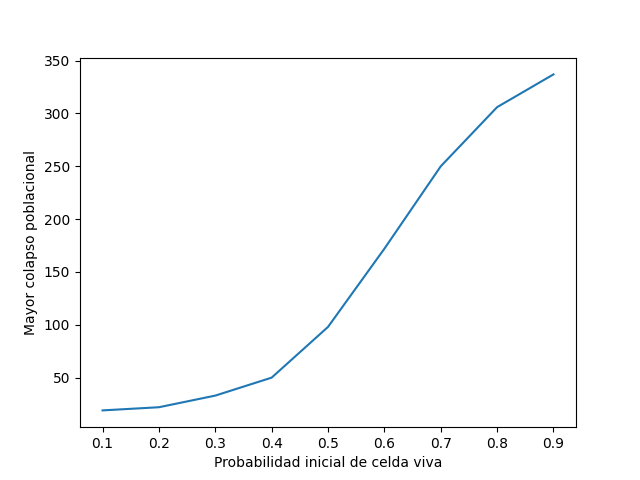
\includegraphics[height=3in]{/Users/victor/Desktop/Figure_1.png}
	\caption{Gráfica con resultados de la simulación.}
	\label{fig:tarea.1}
\end{center}
\end{figure}












\bibliography{ref.Tarea2.bib}
\bibliographystyle{plainnat}

\end{document}
